\graphicspath{{Chapter2/Figs/}}

\chapter{Multi-Omics Factor Analysis (MOFA), a Bayesian model for integration of multi-omics data}

The work described in this chapter results from a collaboration with Wolfgang Huber's group at the EMBL (Heidelberg, Germany). It has been peer-reviewed and published in \cite{Argelaguet2018}.\\
The method was conceived by Florian Buettner, Oliver Stegle and me. I performed most of the mathematical derivations and implementation, but with significant contributions from Damien Arnol and Britta Velten. The CLL data application was led by Britta Velten whereas the single-cell application was led by me, but with joint contributions in either cases. Florian Buettner, Wolfgang Huber and Oliver Stegle supervised the project.\\
The article was jointly written by Britta Velten and me, with contributions from all authors.

\section{Theoretical foundations}

\subsection{Mathematical notation} \label{section:mathematical_notation}

\begin{itemize}[noitemsep]
	\item[--] Matrices are denoted with bold capital letters: $\bfW$
	\item[--] Vectors are denoted with bold non-capital letters: $\bfw$. If the vector comes from a matrix, we will use a single index to indicate the row that it comes from. If two indices are used, the first one corresponds to the row and the second one to the column. The symbol '$:$' denotes the entire row/column. For instance, $\bfw_{i}$ refers to the $i$th row from the $\bfW$ matrix, whereas $\bfw_{:,j}$ refers to the $j$th column.
	\item[--] Scalars are denoted with non-bold and non-capital letters: $w$. If the scalar comes from a 1-dimensional array (a vector), a single subscript will indicate its position in the vector. If the scalar comes from a 2-dimensional array, two indices will be shown at the bottom: the first one corresponding to the row and the second one to the column. For instance, $w_{i,j}$ refers to the value from the $i$th row and the $j$th column of the matrix $\bfW$, and $w_i$ to the $i$th value of the vector $\bfw$. In some cases, higher dimensional arrays (tensors) are used, and the use of multiple indices follows the same rationale.
	\item[--] $\boldzero_k$ is a zero vector of length $k$.
	\item[--] $\I_k$ is the identity matrix with rank $k$.
	\item[--] $\E_q[x]$ denotes the expectation of $x$ under the distribution $q$. When the expectations are taken with respect to the same distribution many times, we will avoid cluttered notation and we will instead use $\la x \ra$.
	\item[--] $\Ndist{x}{\mu,\sigma^2}$: $x$ follows a univariate normal distribution with mean $\mu$ and variance $\sigma^2$.
	\item[--] $\Gdist{x}{a,b}$: $x$ follows a gamma distribution with shape and rate parameters $a$ and $b$.
	\item[--] $\Bdist{x}{a, b}$: $x$ follows a beta distribution with shape and rate parameters $a$ and $b$.
	\item[--] $\text{Ber}(x|\theta)$: $x$ follows a Bernoulli distribution with parameter $\theta$.
	\item[--] $\mathds{1}_0$: Dirac delta function centered at 0.
	\item[--] $Tr(\bfX)$: Trace of the matrix \bfX
\end{itemize}

\subsection{Graphical notation for probabilistic models}

Probabilistic models can be represented in a diagrammatic format (i.e. a graph or a network) that offers a compact visual representation of complicated systems of probability distributions \cite{Bishop2006}. In a graphical model the relationship between the nodes becomes more explicit, namely their conditional independence properties which allow the joint distribution over all variables to be factorised into a series of simpler products involving subsets of variables \cite{Bishop2006}. The basic unit of a network is the node, which represents the different types of variables, including observed variables, unobserved probabilistic variables and unobserved parameters. The nodes are connected by unidirectional edges (arrows) which capture the conditional independence relationship between the variables.

For this thesis we adapted the graphical notations from~\cite{Dietz2010-technical-report-graphs}:

\begin{center}
  \begin{tabular}{m{8cm} m{2cm}}
    Observed variables & \tikz{\node[obs](){$Y$}} \\
    Unobserved probabilistic variables & \tikz{\node[latent](){$\theta$}} \\
    Unobserved parameters & \tikz{\node[latent,double, double distance=1pt](){$\theta$}} \\
    Repetition of node $\theta_n$ for $n\in\llbracket 1;N \rrbracket$ & \tikz{\node[latent](theta){$\theta_n$}; \plate[] {plateN} {(theta)} {$N$};} \\
    Conditional dependency between nodes: $p(Y,\theta) = p(Y|\theta)p(\theta)$ & \tikz{%
            \node[latent]   (theta) {$\theta$};
            \node[obs, xshift=1.5cm] (Y) {$Y$};
            \edge{theta}{Y}}
  \end{tabular}
\end{center}
% For simplicity, fixed hyperparameters are not represented on the graphical model. Unobserved parameters are only represented when optimised together with the unobserved probabilistic variables.



\graphicspath{{Chapter2/Figs/}}

% TO-DO:
% - VBEM algorithm
% - Visualise mean-field assumption by covariance of exact psoterior
% - Describe underestimation of variance
% - Describe coordinate ascent mean-field variational inference. Add algorithm
% 	Finally, CAVI is closely related to Gibbs sampling (Geman and Geman, 1984; Gelfand and Smith, 1990), the classical workhorse of approximate inference. The Gibbs sampler main- tains a realization of the latent variables and iteratively samples from each variable’s com- plete conditional. Equation (18) uses the same complete conditional. It takes the expected log, and uses this quantity to iteratively set each variable’s variational factor.4


\section{Probabilistic modelling}
A scientific model is a simple theoretical representation of a complex natural phenomenon to allow the systematic study of its behaviour. The general idea is that if a model is able to explain some observations, it might be capturing its true underlying laws and can therefore be used to make future predictions.\\ 
In particular, statistical models are a powerful abstraction of nature. They consist on a set of observed variables and a set of (hidden) parameters. The procedure of fitting the parameters using a set of observations is called inference or learning.\\
On of the major challenges of inference when dealing with real data sets is the distinction between signal and noise. An ideal model should learn only the information relevant to gain explanatory power while disregarding the noise. However, this is a non-trivial task in most practical situations. Very complex models will tend to overfit the training data, capturing large amounts of noise and consequently leading to a bad generalisation performance to independent data sets. On the other hand, simplistic models will fit the data poorly, leading to poor explanatory power.\\

The ideas above can be formalised using the framework of probability and statistics.

\subsection{Maximum likelihood inference}
A common approach is to define a statistical model of the data $\bfY$ with a set of parameters $\btheta$ that define a probability distribution $p(\bfY|\btheta)$, called the likelihood function. A simple approach to fit a model is to estimate the parameters $\hat{\btheta}$ that maximise the likelihood:
\[
	\hat{\btheta} = \argmax_{\btheta} p(\bfY|\btheta)
\]
This process is called maximum likelihood learning\cite{Stigler2008,Bishop,Murphy}. However, in this setting there is no penalisation for model complexity, making maximum likelihood solutions prone to overfit in cases where the data is relatively sparse. Generalisations that account for model complexity have been proposed and include regularising terms that shrink parameters to small values. However, these are often particular cases of the more general framework of Bayesian statistics \cite{Hastie,Bishop,Murphy}.

\subsection{Bayesian inference}
In the Bayesian framework, the parameters themselves are treated as random unobserved variables and we aim to obtain probably distributions for $\btheta$, rather than a single point estimate. To do so, prior beliefs are introduced into the model by specifying a prior probability distribution $p(\btheta)$. Then, using Bayes' theorem \cite{Bayes1763}, the prior hypothesis is updated based on the observed data $\bfY$ by means of the likelihood $p(\bfY|\btheta)$ function, which yields a posterior distribution over the parameters:
\[
	p(\btheta|\bfY) = \frac{p(\bfY|\btheta) p(\btheta)}{p(\bfY)}
\]
where $p(\bfY)$ is a constant term called the marginal likelihood, or model evidence \cite{Bishop,Murphy}.\\
The choice of the prior distribution is a key part of Bayesian inference and captures beliefs about the distribution of a variable before the data is taken into account. With asymptotically large sample sizes, the choice of prior has negligible effects on the posterior estimates, but it becomes critical with sparse data \cite{Bishop,Murphy,Gelman2013}.\\
There are two common considerations when defining the prior distributions. The first relates to the incorporation of subjective information, or predefined assumptions, into the model. For example, one could adapt the prior distribution to match the results from previous experiments (i.e. an informative prior). Alternatively, if no information is available one could set set uninformative priors by following maximum entropy principles \cite{Jaynes1968}.\\
The second strategy is based on convenient mathematical properties to make inference tractable. If the likelihood and the prior distributions do not belong to the same family of probability distributions (they are not conjugate) then inference becomes more problematic \cite{Raiffa1961,Bishop,Murphy,Gelman2013}. The existence of conjugate priors is one of the major reasons that justify the widespread use of exponential family distributions in Bayesian models \cite{XX}. An example is the Automatic Relevance Determination prior discussed in [[SECTION X]]. \\

Again, the milestone of Bayesian inference is that an entire posterior probability distribution is obtained for each unobserved variable. This has the clear advantage of naturally handling uncertainity in the estimation of parameters. For instance, when making predictions, a fully Bayesian approach attempts to integrate over all the possible values of all unobserved varaibles, effectively propagating uncertainity across multiple layers of the model. Nevertheless, this calculation is sometimes intractable and one has to resort to point estimates \cite{Bishop,Murphy,Gelman2013}. The simplest approximation to the posterior distribution is to use its mode, which leads to the maximum a posteriori (MAP) estimate:
\[
	\hat{\btheta} = \argmax_{\btheta} p(\btheta) p(\bfY|\btheta) 
\]
This is similar to the maximum likelihood objective function, but with the addition of a term $p(\btheta)$. When the prior dsitribution is chosen smartly, this term penalises for model complexity. Therefore, in contrast to standard (non-penalised) maximum likelihood inference, Bayesian approaches naturally handle the problem of model complexity and overfitting\cite{Bishop,Murphy,Gelman2013}. At the limit of infinite observations, the influence of the prior to the posterior is negligible and the MAP estimate converges towards the Maximum likelihood estimate, hence providing a rational link between the two inference frameworks.\\

\subsection{Deterministic approaches for Bayesian inference}
The central task in Bayesian inference is the direct evaluation of the posterior distributions and/or the computation of expectations with respect to the posterior distributions. In sufficiently complex models, closed-form solutions are not available and one has to resort to approximation schemes, which broadly fall into two classes: stochastic or deterministic \cite{Gelman2013,Blei2016}. 

Stochastic approaches hinge on the generation of samples from the posterior distribution via a Markov Chain Monte Carlo (MCMC) framework. Such techniques have the appealing property of exact results at the asymptotic limit of infinite computational resources. However, in practice, sampling approaches are computationally demanding and suffer from limited scalability to large data sets \cite{Blei2016}.\\
In contrast, deterministic approaches are based on analytical approximations to the posterior distribution, which often lead to biased results. Yet, given the appropriate settings, these approaches are potentially much faster and scalable to large applications \cite{bishop,murphy,Blei2016}.

\subsubsection{Laplace approximation}
The Laplace approximation is probably the simplest of the deterministic tecniques, where the aim is to construct a Gaussian approximation around the mode of the true posterior distribution using a second-order Taylor expansion \cite{Bishop,Murphy}.\\
Suppose $\bfX$ contains all unobserved variables. The true posterior distribution can be written as:
\[
p(\bfX) = \frac{f(\bfX)}{Z}
\]
where $f(\bfX)$ is a function that depends on the unobserved variables and $Z$ is an unknown normalisation constant to ensure that $\int p(\bfX) d\bfX = 1$\\.\\

The second-order Taylor expansion of $\log f(\bfX)$ centered around its (known) mode $\hat{\bfX}$ is: 
\[
	\log f(\bfX) \approx \log f(\hat{\bfX}) - \frac{1}{2} (\bfX-\hat{\bfX})^T \bfA (\bfX-\hat{\bfX})
\]
where $\bfA = \nabla^2 \log f(\hat{\bfX})$ is the Hessian matrix of $\log f(\bfX)$ evaluated at $\hat{\bfX}$.\\
Notice three things. First, the first-order term of the Taylor expansion is zero because $\hat{\bfX}$ is a stationary point. Second, the $\log$ function is monotonically increasing and therefore a maximum of $\log f(\bfX)$ is also a maximum of $f(\bfX)$. Third, the mode of the posterior $p(\bfX)$ must be known, which requires the use of (complex) optimisation algorithms.\\
Taking the exponential in both sides:
\[
	f(\bfX) \approx f(\hat{\bfX}) \exp\{ -\frac{1}{2} (\bfX-\hat{\bfX})^T \bfA (\bfX-\hat{\bfX}) \}
\]
which leads to the following multivariate Gaussian distribution approximation $q(\bfX) = \Ndist{\bfX}{\hat{\bfX},\bfA}$:
\[
	q(\bfX) = \frac{\mid A \mid^{1/2}}{(2\pi^{d/2})} \exp\{ -\frac{1}{2} (\bfX-\hat{\bfX})^T \bfA (\bfX-\hat{\bfX}) \}
\]
where $d$ is the number of unobserved variables. \\
Despite its simplicity, the Laplace approximation is a useful strategy that has been successfully applied in practice. More sophisticated generalisations of the Laplace approximation have also been proposed \cite{Rue2009}.


\subsection{Variational approximation}
Variational inference is a deterministic family of methods that have been receiving widespread attention due to a positive balance between accuracy, speed, and ease of use \cite{Blei_ReviewVB_2017, Zhang2018Arxiv}. The core framework is derived below.\\

In variational inference the true (but intractable) posterior distribution $p(\bfX|\bfY)$ is approximated by a simpler (variational) distribution $q(\bfX|\bTheta)$ where $\bTheta$ are the corresponding parameters. The parameters, which we will omit from the notation, need to be tuned to obtain the closest approximation to the true posterior.\\
The distance between the true distribution and the variational distribution is calculated using the KL divergence:
\[
\KL(q(\bfX)||p(\bfX|\bfY)) = - \int_z q(\bfX) \log \frac{p(\bfX|\bfY)}{q(\bfX)}
\]
Note that the KL divergence is not a proper distance metric, as it is not symmetric. In fact, using the reverse KL divergence $\KL(q(\bfX)||p(\bfX|\bfY))$ defines a different inference framework called expectation propagation \cite{Minka2001}.\\

If we allow any possible choice of $q(\bfX)$, then the minimum of this function occurs when $q(\bfX)$ equals the true posterior distribution $p(\bfX|\bfY)$. Nevertheless, since the true posterior is intractable to compute, this does not lead to any simplification of the problem. Instead, it is necessary to consider a restricted family of distributions $q(\bfX)$ that are tractable to compute and subsequently seek the member of this family for which the KL divergence is minimised.\\

Doing some calculus it can be shown (see \cite{Bishop,Murphy}) that the KL divergence $\KL(q(\bfX)||p(\bfX|\bfY))$ is the difference between the log of the marginal probability of the observations $\log(\bfY)$ and a term $\Lagr(\bfX)$ that is typically called the Evidence Lower Bound (ELBO):
\[
	\KL(q(\bfX)||p(\bfX|\bfY)) = \log(\bfX) - \Lagr(\bfX)
\]
Hence, minimising the KL divergence is equivalent to maximising $\Lagr(\bfX)$ \Cref{fig:ELBO}:
\begin{align} \label{eq_elbo1} \begin{split}
	\Lagr(\bfX) &= \int q(\bfX) \Big( \log \frac{p(\bfX|\bfY)}{q(\bfX)} + \log p(\bfY) \Big) d\bfX \\
	%&= \int \Big( q(\bfX) \log \frac{p(\bfX|\bfY)}{q(\bfX)} + q(\bfX)\log p(\bfY) \Big) d\bfX\\
	%&= \E_q [\log p(\bfX|\bfY)] - \E_q [\log q(\bfX)] + \E_q [\log p(\bfY)] \\
	&= \E_q [\log p(\bfX,\bfY)] - \E_q [\log q(\bfX)]
\end{split} \end{align}
The first term is the expectation of the log joint probability distribution with respect to the variational distribution. The second term is the entropy of the variational distribution.
Importantly, given a simple parametric form of $q(\bfX)$, each of the terms in \Cref{eq_elbo1} can be computed in closed form.\\
In some occasions (see section X), we will use the following form for the ELBO:
\begin{equation} \label{eq_elbo2}
	\Lagr(\bfX) = \E_q [\log p(\bfY|\bfX)] + (\E_q [\log p(\bfX)] - \E_q [\log q(\bfX)])
\end{equation}
where the first term is the expectation of the log likelihood and the second term is the difference in the expectations of the $p$ and $q$ distributions of each hidden variable.\\

In conclusion, variational learning involves minimising the KL divergence between $q(\bfX)$ and $p(\bfX|\bfY)$ by instead maximising $\Lagr(\bfX)$ with respect to the distribution $q(\bfX)$. The following image summarises the general picture of variational learning:

\begin{figure}[H]
	\centering
	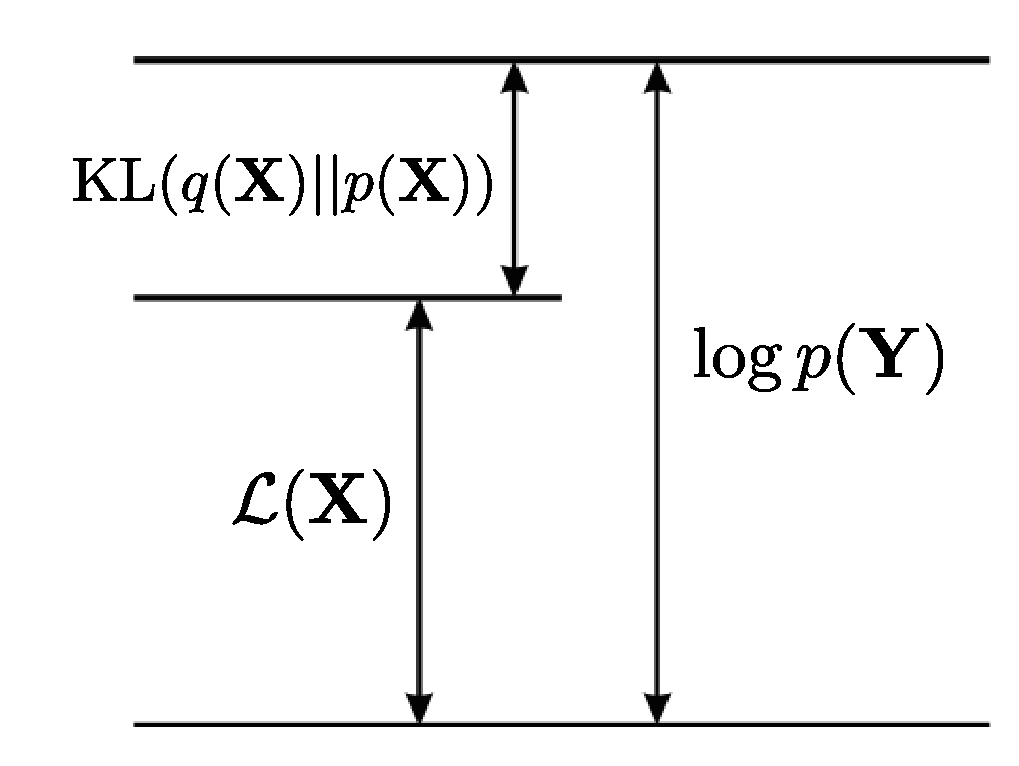
\includegraphics[width=0.35\linewidth]{lower_bound}
	\caption{The quantity $\Lagr(\bfX)$ provides a lower bound on the true log marginal likelihood $\log p(\bfY)$, with the difference being given by the Kullback-Leibler divergence $\KL(q||p)$ between the variational distribution $q(\bfX)$ and the true posterior $p(\bfX|\bfY)$}
	\label{fig:ELBO}
\end{figure}

 Yet, there are several approaches to define $q(\bfX)$. The two most commonly used are called (unparametric) mean-field and (parametric) fixed-form \cite{Zhang2017,Blei2016}.

\subsubsection{Mean-field variational inference}
The most common type of variational Bayes, known as the mean-field approach, assumes that the variational distribution factorises over M disjoint groups of unobserved variables\cite{Saul1996}:
\begin{equation} \label{eq:mean_field}
	q(\bfX) = \prod_{i=1}^{M} q(\bfx_i)
\end{equation}
Typically all unobserved variables are assumed to be independent, extensions that consider structured groups of variables have also been considered\cite{Barber1998,Lawrence1996,Hoffman2014}. Importantly, notice that no parametric assumptions were placed regarding the nature of $q(\bfx_i)$. \\

Evidently, in sufficiently complex models where the unobserved variables have dependencies this family of distributions do not contain the true posterior. Yet, this is a key assumption to obtain an analytical inference scheme that yields surprisingly accurate results \cite{XX}.

Using calculus of variations (see \cite{Bishop,Murphy}), it follows that the optimal distribution $q(\bfX)$ that maximises the lower bound $\Lagr(\bfX)$ is
\begin{equation} \label{eq:optimal}
	\log \hat{q}_i(\bfx_i) = \E_{-i} [\log p(\bfY,\bfX)] + \mathrm{const}
\end{equation}
where $\E_{-i}$ denotes an expectation with respect to the $q$ distributions over all variables $\bfx_j$ except for $\bfx_i$.\\
The additive constant is set by normalising the distribution $\hat{q}_i(\bfz_i)$:
\[
	\hat{q}(\bfx_i) = \frac{\exp(\E_{-i}[\log p(\bfY,\bfX)])}{\int \exp(\E_{-i}[\log p(\bfY,\bfX)]) d\bfX}
\]
While the form of $\hat{q}(\bfx_i)$ is not restricted to a specific parametric form, it can be shown that when using conjugate priors, the distributions $\hat{q}_i(\bfx_i)$ have the same functional form as the priors $\hat{p}(\bfx_i)$. An example is shown in Appendix X, but a detailed mathematical treatment with derivations of multiple examples can be found in \cite{Bishop,Murphy,Zhao2009}.


\subsubsection{(TO-IMPROVE)Fixed-form variational inference}
An alternative and straightforward choice is to directly define the distribution $q(\bfX)$ to be of the same form as the prior distribution $p(\bfX)$, with (variational) parameters $\bTheta$. \\
Importantly, this approach introduces parametric assumptions which only match the mean-field derivation when using conjugate priors. However, for generic models with arbitrary families of distributions, no closed-form variational distributions exist via the mean-field approximation \cite{Zhang2017,Blei2016}. \\
Once the (parametric) choice of $q(\bfX)$ is made, the ELBO can be maximised by optimising the parameters $\bTheta$ via conventional numeric optimisation methods. Hence, while the parametric assumption certainly limits the flexibility of variational distributions, the advantage of this formulation is that it opens up the possibility to use (potentially fast) gradient-based methods for the inference procedure \cite{Hoffman2012,Ranganath2014,Platt2008}.

% Discuss STAN model
% Discuss generic VI


\subsection{Expectation Propagation}
Expectation Propagation (EP) is another deterministic strategy with a similar philosophy as the Variational approach. It is also based on minimising the KL divergence between a variational distribution $q(\bfX)$ and the true posterior $p(\bfX|\bfY)$, but while variational inference minimises $KL(p||q)$, EP maximises the reverse KL-divergence $KL(q||p)$.\\

Interestingly, this simple change leads to an inference scheme with stringkly different properties. This can be understood by inspecting the differences between the two KL divergence formulas:

Variational inference:
\begin{equation} \label{eq:kl_vb}
	\KL(q(\bfX)||p(\bfX|\bfY)) = - \int_z q(\bfX) \log \frac{p(\bfX|\bfY)}{q(\bfX)}
\end{equation}
Expectation propagation:
\begin{equation} \label{eq:kl_ep}
	\KL(p(\bfX|\bfY)||q(\bfX)) = - \int_z p(\bfX|\bfY) \log \frac{q(\bfX)}{p(\bfX|\bfY)}
\end{equation}
In regions of $\bfX$ where the true posterior density $p(\bfX|\bfY)$ is small, setting a large density for $q(\bfX)$ has a much stronger penalisation in \Cref{eq:kl_ep} than in \Cref{eq:kl_vb}, because of the true posterior density being on the denominator. Hence, EP tends to avoid areas where the density $p(\bfX|\bfY)$ is very low, even if it does not correspond to areas of very high-density in $p(\bfX|\bfY)$. In contrast, in \Cref{eq:kl_vb} there is a strong penalty for having low-density $q(\bfX)$ values.\\
As discussed in \cite{Bishop}, the practical consequences of this duality can be observed when the posterior is multi-modal, which tends to be the case for all sufficiently complex bayesian models. In VI, $q(\bfX)$ converges towards ares of high-density in $p(\bfX|\bfY)$, namely local optima, whereas EP tends to capture as much non-zero density regions from $p(\bfX|\bfY)$ as possible, thereby averaging across all optima. In the context of doing predictions, the VI solution is much more desirable than the EP solution, as the average of two good parameter values is not necessarily a good parameter itself.\\
%Furthermore, an important caveat of EP is the lack of theoretical guarantees for convergence \cite{XX}.\\ 
A detailed mathematical treatment of EP, including derivations for specific examples, can be found in \cite{Bishop,Murphy,Minka2001}

\begin{figure}[H]
	\centering
	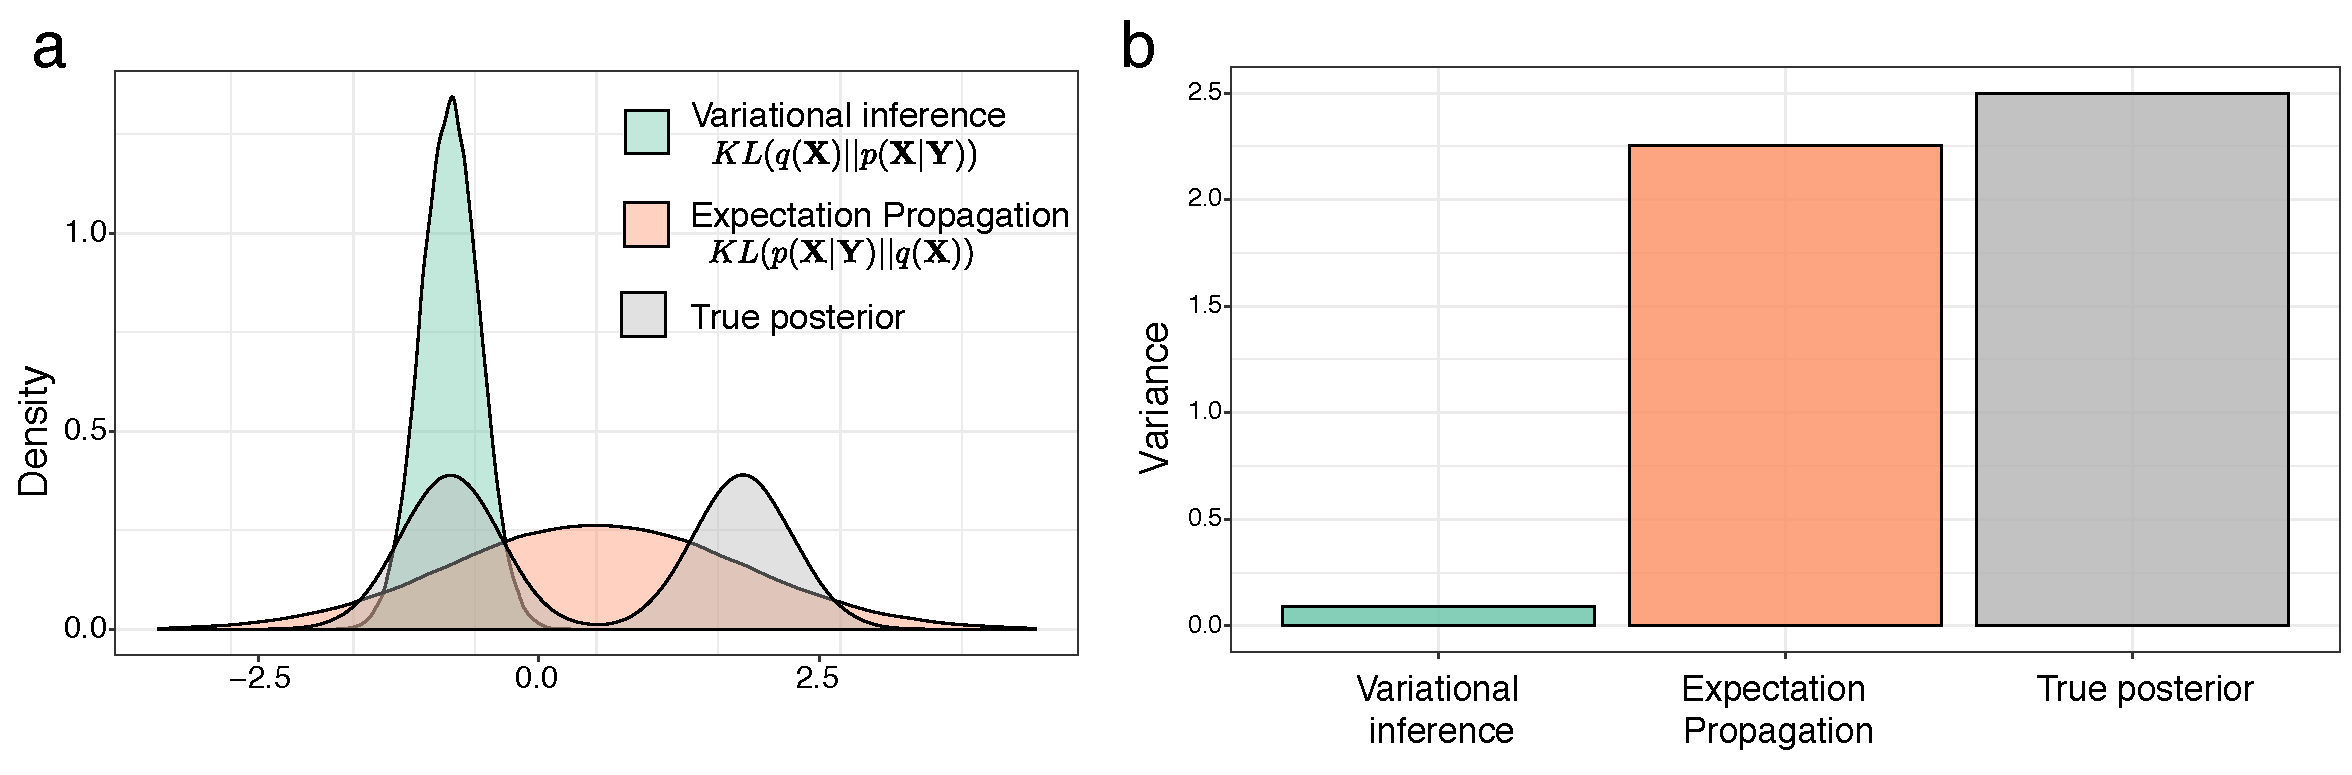
\includegraphics[width=0.9\linewidth]{VB_vs_EP}
	\caption{}
	\label{}
\end{figure}

Following the rationale above, it is easy to predict that variational inference tends to be underestimate the variance of the posterior density. Yet, empirical research have shown that this is acceptable, provided that a good model selection is performed \cite{Blei2017, Blei2006}.\\


\subsubsection{Open perspectives}
Variational inference is growing in popularity for the analysis of big data sets and it has been applied to a myriad of different problems, including genome-wide association studies \cite{Carbonetto2012}, population genetics, \cite{Raj2014}, network analysis \cite{Sanguinetti2006}, computer vision \cite{Likas2004} and natural language processing \cite{Blei2003}.\\

Yet, despite its success, there is room for improvement. First, the theoretical guarantees are not as well developed as in sampling-based MCMC approaches\cite{Blei2016,Zhang2017,Nakajima2007}. For example, although it is surprisingly effective, the mean-field assumption makes strong independence assumptions about the parameters. As we have described, this leads to an underestimation of the true variance in the variational distributions, hence potentially limiting the ability of VI to propagate uncertainity when doing predictions. Additionally, it is not clear in which real case scenarios the dependencies between the parameters becomes so important than the mean-field approximation potentially breaks \cite{XX}. Hence, more generally, an open research problem is understanding what are the statistical properties of the variational posterior with respect to the exact posterior.\\




Alternative strategies beyond the mean-field assumption have been considered by allowing some dependencies between the variables, resulting in \textit{structured} mean-field approximations\cite{Barber1998,Lawrence1996,Hoffman2014}. However, they often lead to very complex (if not intractable) inference frameworks. In this thesis we make use of a structured mean-field assumption for the spike-and-slab prior (see Section X), as initially proposed in \cite{Titsias2011}\\

Another area of extensive research is how to extend the applicability of VI to non-conjugate models. As discussed in section X, the ELBO of non-conjugate models contains intractable integrals and closed-form variational updates cannot be derived. Amenable inference hence requires the use of either stochastic Monte Carlo approximations \cite{XX} or deterministic Taylor/Laplace approximations that introduce additional lower bounds \cite{Zhang2017,Seeger2012,Khan2017}. In this thesis we follow this rationale to derive an inference framework for a model with general likelihoods (see Section X).

% TO-DO: DISCUSS DEEP LEARNING AND VARIATIONAL AUTOENCODERS


 \section{Graphical notations for probabilistic models}

% (COPIED FROM DAMIEN THESIS) Notations were adapted from~\cite{Dietz2010-technical-report-graphs}. The different types of model variables are represented with different types of nodes in the network; nodes repetitions are expressed with plate notations and the conditional dependency between nodes is expressed with directed arrows:
% \begin{center}
%   \begin{tabular}{m{8cm} m{2cm}}
%     Observed variables & \tikz{\node[obs](){$Y$}}\\
%     Unobserved probabilistic variables & \tikz{\node[latent](){$\theta$}}\\
%     Unobserved parameters & \tikz{\node[latent,double, double distance=1pt](){$\theta$}}\\
%     Repetition of node $\theta_n$ for $n\in\llbracket1;N\rrbracket$ & \tikz{\node[latent](theta){$\theta_n$}; \plate[] {plateN} {(theta)} {$N$};}\\
%     Conditional dependency between nodes: $P(Y,\theta) = P(Y|\theta)P(\theta)$ & \tikz{%
%             \node[latent]   (theta) {$\theta$};
%             \node[obs, xshift=1.5cm] (Y) {$Y$};
%             \edge{theta}{Y}}
%   \end{tabular}
% \end{center}
% For simplicity, fixed hyperparameters are not represented on the graphical model. Unobserved parameters are only represented when optimised together with the unobserved probabilistic variables.

\section{Latent variable models for genomics}
With the exponential growth in the use of high-throughput genomics, biological data sets are increasingly high dimensional, both in terms of samples and features. A key principle of biological data sets is that variation between the measured features result from differences in underlying, often unobserved, processess. Such hidden processess, whether biological or technical, affect multiple features in a coordinated fashion due to the existence of interacting gene regulatory networks. This key assumption sets off an entire statistical framework of exploiting the redundancy encoded in the data set to learn the (latent) sources of variation in an unsupervised fashion. This is the aim of dimensionality reduction techniques, or latent variable models (LVMs) \cite{Komili2008, Leek2007, Pournara2007, Dai2017, Genevieve2018, Meng2016}.

\subsection{General mathematical formulation}
Given a dataset $\bfY$ of $N$ samples and $D$ features, LVMs attempt to explain the observations by means of a potentially smaller set of $K$ latent variables, or factors. The mapping between the low-dimensional and the high-dimensional space is performed via a function $f(\bfX|\bTheta)$ that depends on some parameters $\bTheta$.\\

The choice of $f(\bfX|\bTheta)$ is essentially the field of dimensionality reduction. A trade-off exists between complexity and interpretation. While non-linear functions such as deep neural autoencoders provide more explanatory power\cite{}, this leads to a considerable challenge in interpretation. Hence, for most applications where interpretability is important, $f(\bfX|\bTheta)$ is assumed to be linear:
\begin{equation} 
	y_{nd} = \sum_{k=1}^{K} w_{dk}z_{n,k}
\end{equation}
or in matrix form:
\begin{equation} \label{eq:linear_model}
	\mathbf{Y} = \mathbf{Z}\mathbf{W}^{T}
\end{equation}
where $\bfZ \in \R^{N \times K}$ is a matrix that contains the factors (and hence $K<D$). The matrix $\bfW \in \R^{D \times K}$ contains the weights or loadings, which provide the linear mapping between the high-dimensional space (the features) and the low-dimensional space (the latent factors).\\
Note that the aim of the model is to capture the coordinated heterogeneity between features, not to explain differences in their total levels, and hence features are assumed to be centered.\\

The inference procedure consists in learning the values of all unobserved variables, including latent variables and the weights. As we shall demonstrate, different inference schemes and assumptions on the prior distributions lead to significantly different model outputs.

\subsection{Principal component Analysis}
Principal Component Analysis (PCA) is the most popular technique for dimensionality reduction \cite{Hotelling1933,Ringner2008}.\\
Starting from \Cref{eq:linear_model}, two formulations of PCA exist \cite{Bishop}. In the maximum variance formulation, the aim is to infer an orthogonal projection of the data onto a low-dimensional space such that variance explained by the projected data is maximised. For a single principal component, the optimisation problem is:
\begin{align} \label{eq:pca}
	\argmax_{\|\bfw\|=1} & \sum{n=1}^{N} (\bfw_1^T \bfy_n)^2 \\
						 & \bfw_1^T \bfX^T \bfX \bfw \\
						 & \bfw_1^T \bfS \bfw
\end{align}
where $\bfS \in \R^{D \times D}$ is the data covariance matrix defined as $\bfS = \bfX^T \bfX$. The mapping between the high-dimensional space and the low-dimensional space is done again via a vector of loadings $\bfw_1^T$. \\
The $k$-th principal component can be found by subtracting the reconstructed data by the previous $k-1$ principal components from $\bfY$. If we define $\bfz_k=(\bfw_k^T \bfY)$ to be the $k$-th principal component, the optimisation problem is:
\[
	\hat{\bfY} - \bfY - \sum_{k=1}^{K} (\bfz_k \bfw_k^T)
\]
and re-applying \Cref{eq:pca}\\

In its minimum error formulation, the aim is to find an equivalent projection that minimises the mean squared error between the observations and the reconstruction:
\[
	\argmax_{\|\bfw\|=1} \| \bfY - \sum_{k=1}^{K} \bfz_k \bfw_k^T \|^2
\]

% Nice figure here:
% 	http://alexhwilliams.info/itsneuronalblog/2016/03/27/pca/

Solving the two optimisation problems above via Lagrange multipliers leads, remarkably, to the same solution\cite{Bishop}:
\begin{equation}
	\bfS \bfw_k = \lambda_k \bfw_k
\end{equation}
Hence, the loading vectors $\bfw_k$ are equivalent to the eigenvectors of $\bfS$, which can be computed via singular value decomposition.

(EXPLAIN WHY THE TWO SOLUTIONS ARE THE SAME) \\

 
The main strength of PCA relies on its simplicity and closed form solution. Additionally, the linear mapping has the advantage of yielding interpretable loadings, so that inspection of $\bfw_k$ reveals which features are jointly affected by the $k$-th principal component.\\
However, PCA suffers from serious drawbacks when applying it to real data sets. First, biological measurements are inherently noisy, and there is no explicit account of noise in PCA. In practice, high variance components are often asociated with signal whereas low-variance components are assumed to be noise, but an ideal model should explicitly disentangle the uncoordinated (or unexplained) variability that is attributed to noise from the coordinated variability that is characterised as signal. Second, in its original formulation, no missing data is allowed. Third, there is no rationality on how to evaluate the fit and perform model selection. Finally, it does not offer a principled way of modelling prior information about the data.

\subsection{Probabilistic Principal Component Analysis and Factor Analysis}

A generalisation of PCA can be achieved by converting the equation \Cref{eq:linear_model} into a probabilistic framework with an explicit noise term\cite{TippingBishop}:
\begin{equation}
	\bfY = \bfW \bfZ + \bepsilon
\end{equation}
where the weights $\bfW$ are assumed to be fixed parameters. In contrast, the noise $\bepsilon$ and the latent variables $\bfZ$ (the principal components) are assumed to be normally distributed random variables (\cref{fig:pPCA}):
\begin{align}
	p(z_{nk}) &= \Ndist{z_{nk}}{0,1} \\
	p(\epsilon) &= \Ndist {\epsilon}{0,\sigma^2}
\end{align}

All together, this leads to a normally-distributed likelihood:
\begin{equation}
	p(\bfY|\bfW,\bfZ,\sigma) = \Ndist{\bfY}{\bfW \bfZ,\sigma^2 \I}
\end{equation}

\begin{figure}[H] \begin{center}
	% \definecolor{colD}{rgb}{0.2, 0.2, 0.6}
\definecolor{colM}{rgb}{0.0, 0.5, 0.0}
\definecolor{colN}{rgb}{0.5, 0.0, 0.13}
\definecolor{colG}{rgb}{1.0, 0.65, 0.0}
\newcommand\op{0.25}
\colorlet{shadecolor}{black!25}


\begin{tikzpicture}

% Define nodes
\node[obs]   (Y) {$y_{n,d}$};
\node[latent, xshift=-1.5cm, above=of Y, yshift=-0.4cm] (Z) {$z_{n,k}$};
\node[latent, double, double distance=1pt, above=of Y, yshift=0.6cm] (W) {$w_{d,k}$};
\node[latent, double, double distance=1pt, xshift=1.5cm] (Tau) {$\tau$};

% Connect the nodes
\edge {Z,W, Tau} {Y};

% Plates
\plate[] {plateK} {(Z)(W)} {$K$};
\plate[] {plateN} {(Y)(Z)(plateK.south east)(plateK.south west)} {$N$};
\plate[] {plateD} {(Y)(W)(plateK.north east)(plateN.south east)} {$D$};

\end{tikzpicture}
	\label{fig:pPCA}
	\caption{Graphical model for probabilistic PCA. The latent variables are modelled as random variables, whereas the loadings and the noise are modelled as deterministic parameters.}
\end{center} \end{figure}

Importantly, The choice of the distribution for $\epsilon$ implies that the noise of each feature is independent but restricted to have the same magnitude. In practice, this is a limiting assumption, as different features are expected to show different levels of noise. This assumption can be easily relaxed and forms the basis of (probabilistic) Factor Analysis \cite{???}.\\

The inference procedures involves learning the parameters $\bfW$, and $\sigma^2$ and a posterior probability distribution for $\bfZ$.\\
In models that depend on unobserved latent variables, inference can be performed using the iterative Expectation-Maximisation (EM) algorithm \cite{Rubin1983}. In the expectation step, the posterior distribution for $\bfZ$ is computed in closed form (due to conjugacy between the likelihood and the prior), given current estimates for the parameters $\bfW$, and $\sigma^2$. In the maximisation step, the parameters are calculated by maximising the expectation of the joint log likelihood under the posterior distribution of $\bfZ$ found in the E step \cite{TippinBishop}.

Interestingly, the authors showed that the EM solution of probabilistic PCA lies in the same subspace than the traditional PCA solution \cite{ppca}. Yet, the use of a probabilistic framework brings several benefits. First, model selection can be performed by comparing likelihoods across different settings of parameters. Second, missing data can naturally be accounted for by ignoring the missing observations from the likelihood. Finally, the probabilistic formulation sets the core framework for a Bayesian treatment of PCA, enabling a broad range of principled extensions tailored different types of data sets.


\subsection{Bayesian Principal Component Analysis and Bayesian Factor Analysis}

The full Bayesian treatment of PCA requires the specification of prior probability distributions for all unobserved variables:
\begin{align}
	p(z_{nk}) &= \Ndist{z_{nk}}{0,1} \\
	p(w_{dk}) &= \Ndist{w_{dk}}{0,1} \\
	p(\epsilon) &= \Ndist {\epsilon}{\tau} \\
	p(\tau) &= \Gamma{\tau}{a_0,b_0}
\end{align}
where $\tau$ is the precision (inverse of the variance) of the noise term. A generalisation to bayesian Factor Analysis follows by allowing a separate noise term per feature:
\begin{align}
	p(\tau_d) &= \Ndist {\epsilon_d}{0,\tau_d^2} \\
	p(\tau_d) &= \Gamma{\tau_d}{a_0,b_0}
\end{align}
where $a_0$ and $b_0$ are fixed hyperparameters. This results in the following likelihood:
\[
	p(\bfY|\bfW,\bfZ,\btau) = \prod_{n=1}^{N} \prod_{d=1}^{D} \Ndist{y_{nd}}{\bfw_{d,:}^T \bfz_{n,:},\tau_d}
\]

\begin{figure}[H] \begin{center}
	\input{graphical_models/bayesianFA}
	\label{fig:bayesianFA}
	\caption{Graphical model for bayesian Factor Analysis. All unobserved variables are modelled as random variables.}
\end{center} \end{figure}

\subsubsection{Hierarchical priors: Automatic relevance determination}
A key advantage of the full Bayesian treatment, as opposed to the probabilistic PCA model, is that it explicitly captures uncertainity on the estimation of all unobserved variables. Yet, more importantly, the use of (hierarchical) prior distributions allow different modelling assumptions to be encoded, thereby providing a flexible and principled approach to address the limitations of PCA.\\

For example, a major challenge in PCA is how to determine the dimensionality of the latent space (i.e. the number of principle components). The use of hierarchical prior distributions allows the model to introduce sparsity assumptions on the loadings such that only a small subset of (active) factors will contain non-zero leadings.\\
In the context of Factor Analysis, the Automatic Relevance determination (ARD) prior was one of the first ones to be proposed \cite{(David J. C. MacKay, 1994; Neal, 1995; Wipf and Nagarajan, 2008)}:
\begin{equation*} \label{eq:ard}
	P(\bfW|\balpha) = \prod_{k=1}^{K} \Ndist{\bfw_{:,k}}{0,\frac{1}{\alpha_{k}}\I_{D}}\\
	\qquad\qquad
	P(\balpha) = \prod_{k=1}^{K} \Gdist{\alpha_k}{a_0^\alpha, b_0^\alpha}\\
\end{equation*}
The aim of this prior is two-fold. First, the zero-mean normal distribution specifies that, \textit{a priori}, no information is available and all features are inactive. When exposed to some data, the posterior distribution for $\bfW$ will be estimated by weighting the contribution from the likelihood and from the prior, hence allowing each feature to escape from the initial zero.\\
Second, performing inference on the variable $\balpha$ enables the model to automatically learns the number of factors. To understand this, let us assume that only $K=5$ true factors exist, but the model is initialised with $K=20$ factors. In such case, inactive factors can be prunned out by driving the corresponding $\alpha_k$ to infinity. In turn, this causes the posterior $p(\bfW_{:,k}|\bfY)$ to be sharply peaked at zero \Cref{fig:ard}, resulting in the full inactivation of all loadings \Cref{fig:hinton}. 

\begin{figure}[H] \begin{center}
	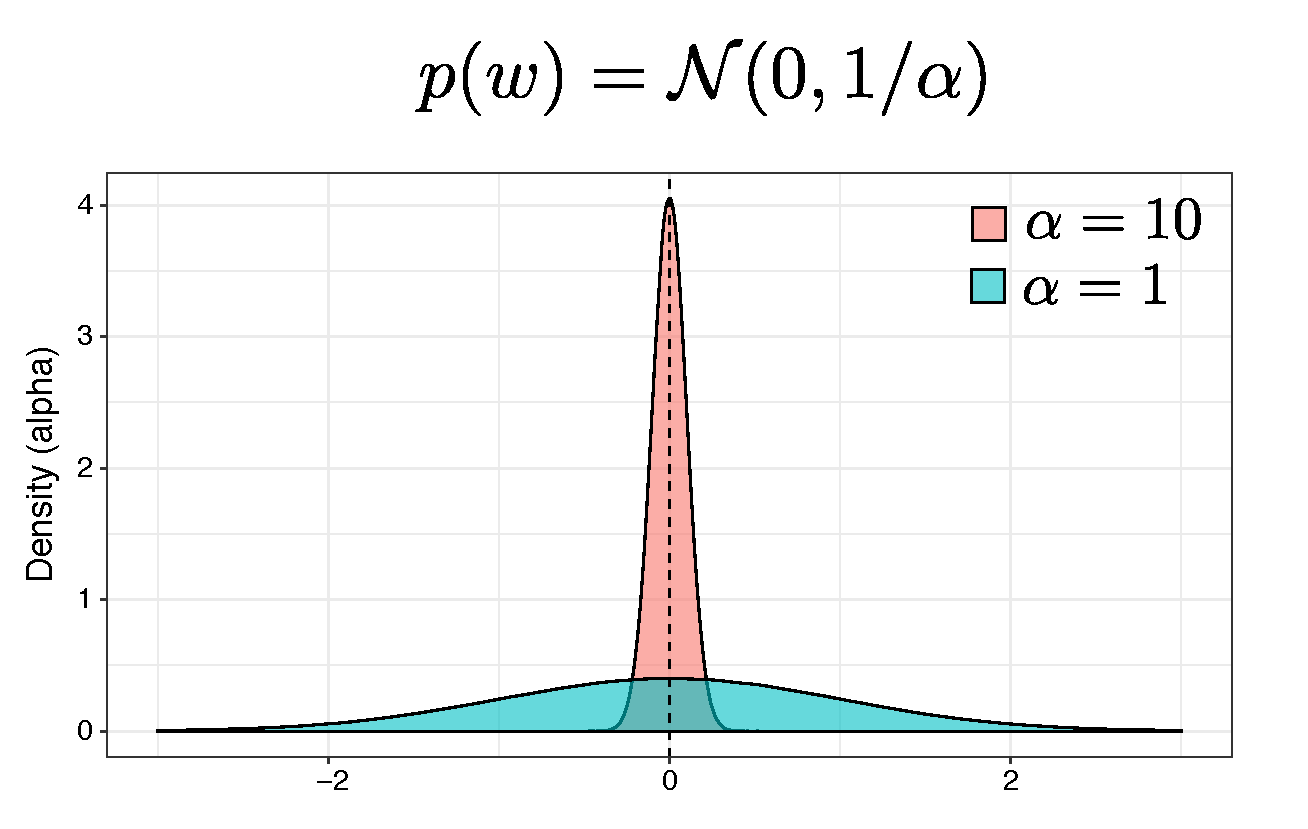
\includegraphics[width=0.8\textwidth]{Chapter2/Figs/ard}
	\caption{}
	\label{fig:ard}
\end{center} \end{figure}

\begin{figure}[H] \begin{center}
	\includegraphics[width=0.8\textwidth]{Chapter2/Figs/hinton}
            \caption[Hinton plot of the loading matrix for a bayesian Factor Analysis model with an ARD prior]{Hinton plots display the values of the loading matrix, similar to a heatmap, where bigger squares depict larger loadings. Shown are the Hinton plots for (a) the true weights, (b) the infered weights by a Factor Analysis model with no ARD prior (middle), and (c) the infered weights by a Factor Analysis model with ARD prior per factor.\\
            This figure was generated using simulated data with $N=100$ samples, $D=10$ features and $K=3$ factors.}
	\label{fig:hinton}
\end{center} \end{figure}

\subsubsection{Hierarchical priors: Spike-and-slab prior}
Sparse extensions of the Bayesian factor analysis model have been proposed as a regularisation mechanism but also to model inherent assumptions regarding the sparse nature of biological data \cite{West2003,Stegle2012,Gao2013}. In practice, the variability observed in biological data sets is driven both by strong technical factors (i.e. batch effects) and by relatively weak biological factors, driven by potentially small gene regulatory networks \cite{Gao2013}. Hence, a realistic factor analysis model should be learn both types of factors. The ARD prior proposed in \Cref{eq:ard} allows entire factors to be dropped out from the model, but it provides a weak degree of regularisation in the feature loadings of active factors.\\
A sparse generalisation of the bayesian Factor Analysis model can be achieved by combining the ARD prior with a spike-and-slab prior \cite{(Mitchell and Beauchamp, 1988) }:
\begin{equation}
	p(w_{d,k} \mid \alpha_k,\theta_k) = (1-\theta_k) \mathds{1}_0(w_{d,k}) + \theta_k \Ndist{w_{d,k}}{0, \alpha_k^{-1}}
\end{equation}

\begin{figure}[H] \begin{center}
	\begin{tikzpicture}

% Define nodes
\node[obs]   (Y) {$y_{n,d}$};
\node[latent, above=of Y, xshift=-1.5cm] (Z) {$z_{n,k}$};
\node[latent, above=of W, xshift=-0.75cm] (Theta) {$\theta_{k}$};
\node[latent, above=of W, xshift=0.75cm] (Alpha) {$\alpha_{k}$};
\node[latent, above=of Y, xshift=1.5cm] (W) {$w_{d,k}$};
\node[latent, xshift=1.5cm] (Tau) {$\tau_{d}$};

% Connect the nodes
\edge {Theta, Alpha} {W};
\edge {Z, W, Tau} {Y};

% Plates
\plate[] {plateK} {(Z)(W)(Theta)(Alpha)} {$K$};
% \plate[] {plateN} {(Y)(Z)(plateK.north west)} {$N$};
\plate[] {plateN} {(Y)(Z)} {$N$};
\plate[] {plateD} {(Y)(W)(Tau)(plateK.south east) (plateN.south east) (plateN.north east)} {$D$};

\end{tikzpicture}
	\label{fig:bayesianFA}
	\caption{Graphical model for bayesian sparse Factor Analysis}
\end{center} \end{figure}

The spike-and-slab prior is effectively a mixture model where features are sampled from a zero-inflated gaussian distribution, where $\theta \in (0,1)$ dictates the level of sparsity (i.e. how many active features). A value of $\theta_k$ close to $0$ implies that most of the weights of factor $k$ are shrinked to $0$ (i.e. a sparse factor), whereas a value of $\theta_k$ close to $1$ implies that most of the weights are non-zero (i.e. dense factors). Hence, by learning $\theta_k$ from the data, the model naturally accounts for combinations of sparse and dense factors. As in \Cref{eq:ard}, $\alpha_k$ provides the ARD regularisation required to prune inactive factors. \\


\subsubsection{Inference}
In a fully Bayesian setting, the inference procedure corresponds to learning the posterior distributions for each unobserved variable. However, applying Bayes rule yields an analytically intractable solution, and approximate methods are required. This is discussed in Chapter X.
